\documentclass[12pt,twoside]{article}

\newcommand{\reporttitle}{M2R2}
\usepackage{autobreak}
\newcommand{\reporttype}{Coursework}
\newcommand{\rn}{$\mathbb{R}^n$}
\allowdisplaybreaks
% include files that load packages and define macros
%%%%%%%%%%%%%%%%%%%%%%%%%%%%%%%%%%%%%%%%%
% University Assignment Title Page 
% LaTeX Template
% Version 1.0 (27/12/12)
%
% This template has been downloaded from:
% http://www.LaTeXTemplates.com
%
% Original author:
% WikiBooks (http://en.wikibooks.org/wiki/LaTeX/Title_Creation)
%
% License:
% CC BY-NC-SA 3.0 (http://creativecommons.org/licenses/by-nc-sa/3.0/)
% 
% Instructions for using this template:
% This title page is capable of being compiled as is. This is not useful for 
% including it in another document. To do this, you have two options: 
%
% 1) Copy/paste everything between \begin{document} and \end{document} 
% starting at \begin{titlepage} and paste this into another LaTeX file where you 
% want your title page.
% OR
% 2) Remove everything outside the \begin{titlepage} and \end{titlepage} and 
% move this file to the same directory as the LaTeX file you wish to add it to. 
% Then add \input{./title_page_1.tex} to your LaTeX file where you want your
% title page.
%
%----------------------------------------------------------------------------------------
%	PACKAGES AND OTHER DOCUMENT CONFIGURATIONS
%----------------------------------------------------------------------------------------
\usepackage{ifxetex}
\usepackage{textpos}
\usepackage{natbib}
\usepackage{kpfonts}
\usepackage[a4paper,hmargin=2.8cm,vmargin=2.0cm,includeheadfoot]{geometry}
\usepackage{ifxetex}
\usepackage{stackengine}
\usepackage{tabularx,longtable,multirow,subfigure,caption}%hangcaption
\usepackage{fncylab} %formatting of labels
\usepackage{fancyhdr}
\usepackage{color}
\usepackage[tight,ugly]{units}
\usepackage{url}
\usepackage{float}
\usepackage[english]{babel}
\usepackage{amsmath}
\usepackage{graphicx}
\usepackage[colorinlistoftodos]{todonotes}
\usepackage{dsfont}
\usepackage{epstopdf} % automatically replace .eps with .pdf in graphics
\usepackage{natbib}
\usepackage{backref}
\usepackage{array}
\usepackage{latexsym}
\usepackage{etoolbox}

\usepackage{enumerate} % for numbering with [a)] format 



\ifxetex
\usepackage{fontspec}
\setmainfont[Scale=.8]{OpenDyslexic-Regular}
\else
\usepackage[pdftex,pagebackref,hypertexnames=false,colorlinks]{hyperref} % provide links in pdf
\hypersetup{pdftitle={},
  pdfsubject={}, 
  pdfauthor={\reportauthor},
  pdfkeywords={}, 
  pdfstartview=FitH,
  pdfpagemode={UseOutlines},% None, FullScreen, UseOutlines
  bookmarksnumbered=true, bookmarksopen=true, colorlinks,
    citecolor=black,%
    filecolor=black,%
    linkcolor=black,%
    urlcolor=black}
\usepackage[all]{hypcap}
\fi

\usepackage{tcolorbox}

% various theorems


\newtheorem{lemma}{Lemma}
\newtheorem{proposition}[lemma]{Proposition}
\newtheorem{theorem}[lemma]{Theorem}
\newtheorem{corollary}[lemma]{Corollary}
\newtheorem{definition}[lemma]{Definition}
\newtheorem{examp}[lemma]{Example}
\newtheorem{remark}[lemma]{Remark}

\newenvironment{proof}
 {\begin{trivlist}\item[\textit{ Proof:}]\,}
 {$\Box$\end{trivlist}}
\numberwithin{lemma}{section}
\newenvironment{example}[1]{\begin{examp} #1: % \newline \rm 
\normalfont }{\end{examp}}
% example-environment
\newenvironment{example}[1][]
{ 
\vspace{4mm}
\noindent\makebox[\linewidth]{\rule{\hsize}{1.5pt}}
\textbf{Example #1}\\
}
{ 
\noindent\newline\makebox[\linewidth]{\rule{\hsize}{1.0pt}}
}
\newenvironment{claim}[1]{\par\noindent\underline{Claim:}\space#1}{}
\newenvironment{claimproof}[1]{\par\noindent\underline{Proof:}\space#1}{\hfill $\blacksquare$}


%\renewcommand{\rmdefault}{pplx} % Palatino
% \renewcommand{\rmdefault}{put} % Utopia

\ifxetex
\else
\renewcommand*{\rmdefault}{bch} % Charter
\renewcommand*{\ttdefault}{cmtt} % Computer Modern Typewriter
%\renewcommand*{\rmdefault}{phv} % Helvetica
%\renewcommand*{\rmdefault}{iwona} % Avant Garde
\fi

\setlength{\parindent}{0em}  % indentation of paragraph

\setlength{\headheight}{14.5pt}
\pagestyle{fancy}
\fancyfoot[ER,OL]{\thepage}%Page no. in the left on
                                %odd pages and on right on even pages
\fancyfoot[OC,EC]{\sffamily }
\renewcommand{\headrulewidth}{0.1pt}
\renewcommand{\footrulewidth}{0.1pt}
\captionsetup{margin=10pt,font=small,labelfont=bf}


%--- chapter heading

\def\@makechapterhead#1{%
  \vspace*{10\p@}%
  {\parindent \z@ \raggedright %\sffamily
        %{\Large \MakeUppercase{\@chapapp} \space \thechapter}
        %\\
        %\hrulefill
        %\par\nobreak
        %\vskip 10\p@
    \interlinepenalty\@M
    \Huge \bfseries 
    \thechapter \space\space #1\par\nobreak
    \vskip 30\p@
  }}

%---chapter heading for \chapter*  
\def\@makeschapterhead#1{%
  \vspace*{10\p@}%
  {\parindent \z@ \raggedright
    \sffamily
    \interlinepenalty\@M
    \Huge \bfseries  
    #1\par\nobreak
    \vskip 30\p@
  }}
  



% %%%%%%%%%%%%% boxit
\def\Beginboxit
   {\par
    \vbox\bgroup
	   \hrule
	   \hbox\bgroup
		  \vrule \kern1.2pt %
		  \vbox\bgroup\kern1.2pt
   }

\def\Endboxit{%
			      \kern1.2pt
		       \egroup
		  \kern1.2pt\vrule
		\egroup
	   \hrule
	 \egroup
   }	

\newenvironment{boxit}{\Beginboxit}{\Endboxit}
\newenvironment{boxit*}{\Beginboxit\hbox to\hsize{}}{\Endboxit}



\allowdisplaybreaks

\makeatletter
\newcounter{elimination@steps}
\newcolumntype{R}[1]{>{\raggedleft\arraybackslash$}p{#1}<{$}}
\def\elimination@num@rights{}
\def\elimination@num@variables{}
\def\elimination@col@width{}
\newenvironment{elimination}[4][0]
{
    \setcounter{elimination@steps}{0}
    \def\elimination@num@rights{#1}
    \def\elimination@num@variables{#2}
    \def\elimination@col@width{#3}
    \renewcommand{\arraystretch}{#4}
    \start@align\@ne\st@rredtrue\m@ne
}
{
    \endalign
    \ignorespacesafterend
}
\newcommand{\eliminationstep}[2]
{
    \ifnum\value{elimination@steps}>0\leadsto\quad\fi
    \left[
        \ifnum\elimination@num@rights>0
            \begin{array}
            {@{}*{\elimination@num@variables}{R{\elimination@col@width}}
            |@{}*{\elimination@num@rights}{R{\elimination@col@width}}}
        \else
            \begin{array}
            {@{}*{\elimination@num@variables}{R{\elimination@col@width}}}
        \fi
            #1
        \end{array}
    \right]
    & 
    \begin{array}{l}
        #2
    \end{array}
    &%                                    moved second & here
    \addtocounter{elimination@steps}{1}
}
\makeatother

%% Fast macro for column vectors
\makeatletter  
\def\colvec#1{\expandafter\colvec@i#1,,,,,,,,,\@nil}
\def\colvec@i#1,#2,#3,#4,#5,#6,#7,#8,#9\@nil{% 
  \ifx$#2$ \begin{bmatrix}#1\end{bmatrix} \else
    \ifx$#3$ \begin{bmatrix}#1\\#2\end{bmatrix} \else
      \ifx$#4$ \begin{bmatrix}#1\\#2\\#3\end{bmatrix}\else
        \ifx$#5$ \begin{bmatrix}#1\\#2\\#3\\#4\end{bmatrix}\else
          \ifx$#6$ \begin{bmatrix}#1\\#2\\#3\\#4\\#5\end{bmatrix}\else
            \ifx$#7$ \begin{bmatrix}#1\\#2\\#3\\#4\\#5\\#6\end{bmatrix}\else
              \ifx$#8$ \begin{bmatrix}#1\\#2\\#3\\#4\\#5\\#6\\#7\end{bmatrix}\else
                 \PackageError{Column Vector}{The vector you tried to write is too big, use bmatrix instead}{Try using the bmatrix environment}
              \fi
            \fi
          \fi
        \fi
      \fi
    \fi
  \fi 
}  
\makeatother

\robustify{\colvec}

\usepackage{xargs}                      % Use more than one optional parameter in a new commands
\usepackage[pdftex,dvipsnames]{xcolor}  % Coloured text etc.
% 
\usepackage[colorinlistoftodos,prependcaption,textsize=tiny]{todonotes}
\newcommandx{\unsure}[2][1=]{\todo[linecolor=red,backgroundcolor=red!25,bordercolor=red,#1]{#2}}
\newcommandx{\change}[2][1=]{\todo[linecolor=blue,backgroundcolor=blue!25,bordercolor=blue,#1]{#2}}
\newcommandx{\info}[2][1=]{\todo[linecolor=green,backgroundcolor=green!25,bordercolor=green,#1]{#2}}
\newcommandx{\improvement}[2][1=]{\todo[linecolor=purple,backgroundcolor=purple!25,bordercolor=purple,#1]{#2}}
\newcommandx{\thiswillnotshow}[2][1=]{\todo[disable,#1]{#2}}
%

%%% Local Variables: 
%%% mode: latex
%%% TeX-master: "notes"
%%% End: 

 % various packages needed for maths etc.
% quick way of adding a figure
\newcommand{\fig}[3]{
 \begin{center}
 \scalebox{#3}{\includegraphics[#2]{#1}}
 \end{center}
}

%\newcommand*{\point}[1]{\vec{\mkern0mu#1}}
\newcommand{\ci}[0]{\perp\!\!\!\!\!\perp} % conditional independence
\newcommand{\point}[1]{{#1}} % points 
\renewcommand{\vec}[1]{{\boldsymbol{{#1}}}} % vector
\newcommand{\mat}[1]{{\boldsymbol{{#1}}}} % matrix
\newcommand{\R}[0]{\mathds{R}} % real numbers
\newcommand{\Z}[0]{\mathds{Z}} % integers
\newcommand{\N}[0]{\mathds{N}} % natural numbers
\newcommand{\nat}[0]{\mathds{N}} % natural numbers
\newcommand{\Q}[0]{\mathds{Q}} % rational numbers
\ifxetex
\newcommand{\C}[0]{\mathds{C}} % complex numbers
\else
\newcommand{\C}[0]{\mathds{C}} % complex numbers
\fi
\newcommand{\tr}[0]{\text{tr}} % trace
\renewcommand{\d}[0]{\mathrm{d}} % total derivative
\newcommand{\inv}{^{-1}} % inverse
\newcommand{\id}{\mathrm{id}} % identity mapping
\renewcommand{\dim}{\mathrm{dim}} % dimension
\newcommand{\rank}[0]{\mathrm{rk}} % rank
\newcommand{\determ}[1]{\mathrm{det}(#1)} % determinant
\newcommand{\scp}[2]{\langle #1 , #2 \rangle}
\newcommand{\kernel}[0]{\mathrm{ker}} % kernel/nullspace
\newcommand{\img}[0]{\mathrm{Im}} % image
\newcommand{\idx}[1]{{(#1)}}
\DeclareMathOperator*{\diag}{diag}
\newcommand{\E}{\mathds{E}} % expectation
\newcommand{\var}{\mathds{V}} % variance
\newcommand{\gauss}[2]{\mathcal{N}\big(#1,\,#2\big)} % gaussian distribution N(.,.)
\newcommand{\gaussx}[3]{\mathcal{N}\big(#1\,|\,#2,\,#3\big)} % gaussian distribution N(.|.,.)
\newcommand{\gaussBig}[2]{\mathcal{N}\left(#1,\,#2\right)} % see above, but with brackets that adjust to the height of the arguments
\newcommand{\gaussxBig}[3]{\mathcal{N}\left(#1\,|\,#2,\,#3\right)} % see above, but with brackets that adjust to the height of the arguments
\DeclareMathOperator{\cov}{Cov} % covariance (matrix) 
\ifxetex
\renewcommand{\T}[0]{^\top} % transpose
\else
\newcommand{\T}[0]{^\top}
\fi
% matrix determinant
\newcommand{\matdet}[1]{
\left|
\begin{matrix}
#1
\end{matrix}
\right|
}



%%% various color definitions
\definecolor{darkgreen}{rgb}{0,0.6,0}

\newcommand{\blue}[1]{{\color{blue}#1}}
\newcommand{\red}[1]{{\color{red}#1}}
\newcommand{\green}[1]{{\color{darkgreen}#1}}
\newcommand{\orange}[1]{{\color{orange}#1}}
\newcommand{\magenta}[1]{{\color{magenta}#1}}
\newcommand{\cyan}[1]{{\color{cyan}#1}}


% redefine emph
\renewcommand{\emph}[1]{\blue{\bf{#1}}}

% place a colored box around a character
\gdef\colchar#1#2{%
  \tikz[baseline]{%
  \node[anchor=base,inner sep=2pt,outer sep=0pt,fill = #2!20] {#1};
    }%
}%
 % short-hand notation and macros

\usepackage{setspace}
\doublespacing
%\theoremstyle{definition}
\begin{document}
% front page
\begin{titlepage}

\newcommand{\HRule}{\rule{\linewidth}{0.5mm}} % Defines a new command for the horizontal lines, change thickness here


%----------------------------------------------------------------------------------------
%	LOGO SECTION
%----------------------------------------------------------------------------------------

\includegraphics[width = 4cm]{./figures/imperial}\\[0.5cm] 

\begin{center} % Center remainder of the page

%----------------------------------------------------------------------------------------
%	HEADING SECTIONS
%----------------------------------------------------------------------------------------
\textsc{\LARGE \reporttype}\\[1.5cm] 
\textsc{\Large Imperial College London}\\[0.5cm] 
\textsc{\large Department of Mathematics and Computing}\\[0.5cm] 
%----------------------------------------------------------------------------------------
%	TITLE SECTION
%----------------------------------------------------------------------------------------

\HRule \\[0.4cm]
{ \huge \bfseries \reporttitle}\\ % Title of your document
\HRule \\[1.5cm]
\end{center}
%----------------------------------------------------------------------------------------
%	AUTHOR SECTION
%----------------------------------------------------------------------------------------

%\begin{minipage}{0.4\hsize}
\textit{Authors:} \\
Ameena Hassan (CID: 01506240) \\
Dingxuan Zhang (CID: 01718078) \\
Shumin Jiang (CID: 01734086) \\
Jiacheng Xu (CID: 01708919) \\
\\
\\
\textit{Supervisor: }\\
Dr. Marie-Amèlie Lawn

\vspace{2cm}
\makeatletter
Date: \@date 

\vfill % Fill the rest of the page with whitespace



\makeatother


\end{titlepage}


\newpage https://www.overleaf.com/project/60ae381fa7eddee7eca030be
\tableofcontents{}
\newpage
%\listoftodos[Notes]
%%%%%%%%%%%%%%%%%%%%%%%%%%%% Main document
\section{Introduction}

% \todo[inline]{Example: The original todo note without changed colours.\newline Here's another line.}
% \improvement[inline]{We can fill this out near the end.}
% This is a template for coursework submission. Many macros and definitions can be found in \texttt{notation.tex}. This document is not an introduction to LaTeX. General advice if get stuck: Use your favorite search engine. A great source is also \mbox{\url{https://en.wikibooks.org/wiki/LaTeX}}.

The main goal of this project is to give a short introduction on manifolds and homogeneous space, and give intuitive examples of each definition, so that we can build up the concepts slowly. The second section lists very basic definitions that we are going to refer later. Section 3 and 4 give us properties of manifolds and how group actions act on them. Section 5 and 6 focus on homogeneous spaces and how they are related to fiber bundles. And finally, section 7 talks about why homogeneous spaces are important and how it relates to other areas of mathematics.

\section{Brief definitions}
Most of the results derived in this project is based on considering manifolds as the topological space being studied, which may be an abstract concept to work on from the beginning. Therefore we wish to introduce a few 'basic' definitions which is defined on the general topological space, and take some intuitive examples of the spaces and subspaces that we know about, for instance, the Euclidean space \rn. Some of these definitions are already covered in the Groups and Rings module, but we will define them in an alternative way.

\input{Definition_subpages/1_group_actions_defs}

\begin{example}{}
\begin{enumerate}
    \item The symmetric group $S(n)$ acts on the set $\{1,2,...,n\}$ by the various permutation maps;
    \item The multiplicative group $R^{\ast}$ acts on the Euclidean space \rn\ by the scalar multiplication map.
\end{enumerate}
\end{example} 
We can now also define transitive group actions, which will be the type of group actions we focus on in this project.
\begin{definition}
A group action $G \times X \rightarrow X$ is called a \textbf{transitive} action if there exists $x\in X$ such that $X = G\cdot x = \{g\cdot x\ |\ g\in G\}$, where $G\cdot x$ is called the \mathbf{G-orbit of x}.
\end{definition}

\begin{definition}
${S^{n}}\subset$  $\mathbb{R}^{n+1}$ is defined as the set: $\{ x\in\mathbb{R}^{n+1}: \|x\| = 1 \}$, and can also be called the \textbf{n-sphere}.
\end{definition}

\begin{example}{}
There are 9 transitive group actions on a sphere $S^n$ displayed in the table below: \cite{einstein mfd}\\
\\
\begin{tabularx}{1\textwidth} { 
  | >{\centering\arraybackslash}X 
  | >{\centering\arraybackslash}X 
  | >{\centering\arraybackslash}X 
  | >{\centering\arraybackslash}X |}
 \hline
 Group & SO(n) & U(n), SU(n) & Sp(n)Sp(1), Sp(n)U(1), Sp(n) \\
 \hline
 Sphere  & S^{n-1}  & S^{2n-1} & S^{4n-1} \\
\hline
\end{tabularx}\\
\begin{center}
\begin{tabularx}{0.5\textwidth} { 
  | >{\centering\arraybackslash}X 
  | >{\centering\arraybackslash}X 
  | >{\centering\arraybackslash}X  |}
 \hline
 G_2 & Spin(7) & Spin(9) \\
 \hline
 S^6  & S^7  & S^{15} \\
\hline
\end{tabularx}
\end{center}
We 
now aim to show that the special orthogonal group $SO(n+1)$ is a transitive group action on $S^n$. To prove this, we will have to prove a few things about topological spaces, specifically, manifolds. It turns out that $S^{n}$ is also a manifold, and we can use some of these results to prove $SO(n+1)$ acts transitively on $S^{n}$.
\end{example}

\subsection{Homeomorphism and diffeomorphism}
In this subsection we shall define two concepts to describe maps between topological spaces and they will be referred frequently throughout the rest of the project.
\begin{definition}
A \textbf{homeomorphism} between two topological spaces $X,Y$ is a continuous bijection $f: X \rightarrow Y$ whose inverse is also continuous.
\end{definition}

\begin{definition}
A \textbf{diffeomorphism} is a smooth homeomorphism whose inverse is also smooth.
\end{definition}

\subsection{Charts and atlases}

\begin{definition}
A \textbf{chart} $(U,\varphi)$ for a topological space $X$ is a homeomorphism $\varphi$ from an open $U$ is a subset of $X$ to an open subset $\tilde{U}$ contained in \rn, that is $\varphi : U \rightarrow \tilde{U}$.
\end{definition}

\begin{definition}
An \textbf{atlas} for a topological space $X$ is the collection of charts for $X$ which covers $X$.
\end{definition}

\begin{figure}[tb]
\centering
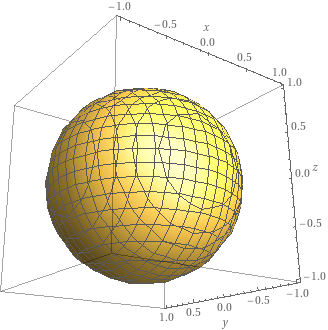
\includegraphics[width=60mm]{3d sphere.png} 
\caption{An atlas of the 2-sphere}
\end{figure}

\begin{example}{}
\label{2sphere}
Consider the 2-sphere $S^2$, better known as the unit sphere on the $xyz-$ Cartesian coordinates. There are infinite ways of splitting charts for a space, and this is not usually discussed. Figure 1 shows the most intuitive  way, by
 splitting the sphere into 6 open hemispheres and projecting them into 6 squares. Taking the example of the open hemisphere in the front (the equator not included), each point is uniquely determined by the $x-$ and $z-$ coordinates, therefore the map from the hemisphere to the subspace of $\mathbb{R}^2$: $\{(x,z)\ |\ x \in (-1,1), z \in (-1,1)\}$ is a continuous bijection, where the map can be expressed mathematically as $\varphi_{front}(x,y,z) = (x,z)$ (here continuity can be obtained by taking partial derivatives and bijectivity is obvious). By similar argument we can construct homeomorphisms for other hemispheres:
\\
$\varphi_{back}(x,y,z) = (x,z), \ \varphi_{top}(x,y,z) = (x,y), \ \varphi_{bottom}(x,y,z) = (x,y), \ \varphi_{left}(x,y,z) = (y,z),\\
\ \varphi_{right}(x,y,z) = (y,z)$
\\
Note that the 4 open hemispheres 'front', 'back', 'top' and 'bottom' does not cover the whole sphere, as the two points $(0,1,0)$ and $(0,-1,0)$ are not included due to the openness of the subset hence the remaining 2 hemispheres are essential to construct an atlas for $S^2$.\\
\end{example}

\begin{figure}[tb]
\centering
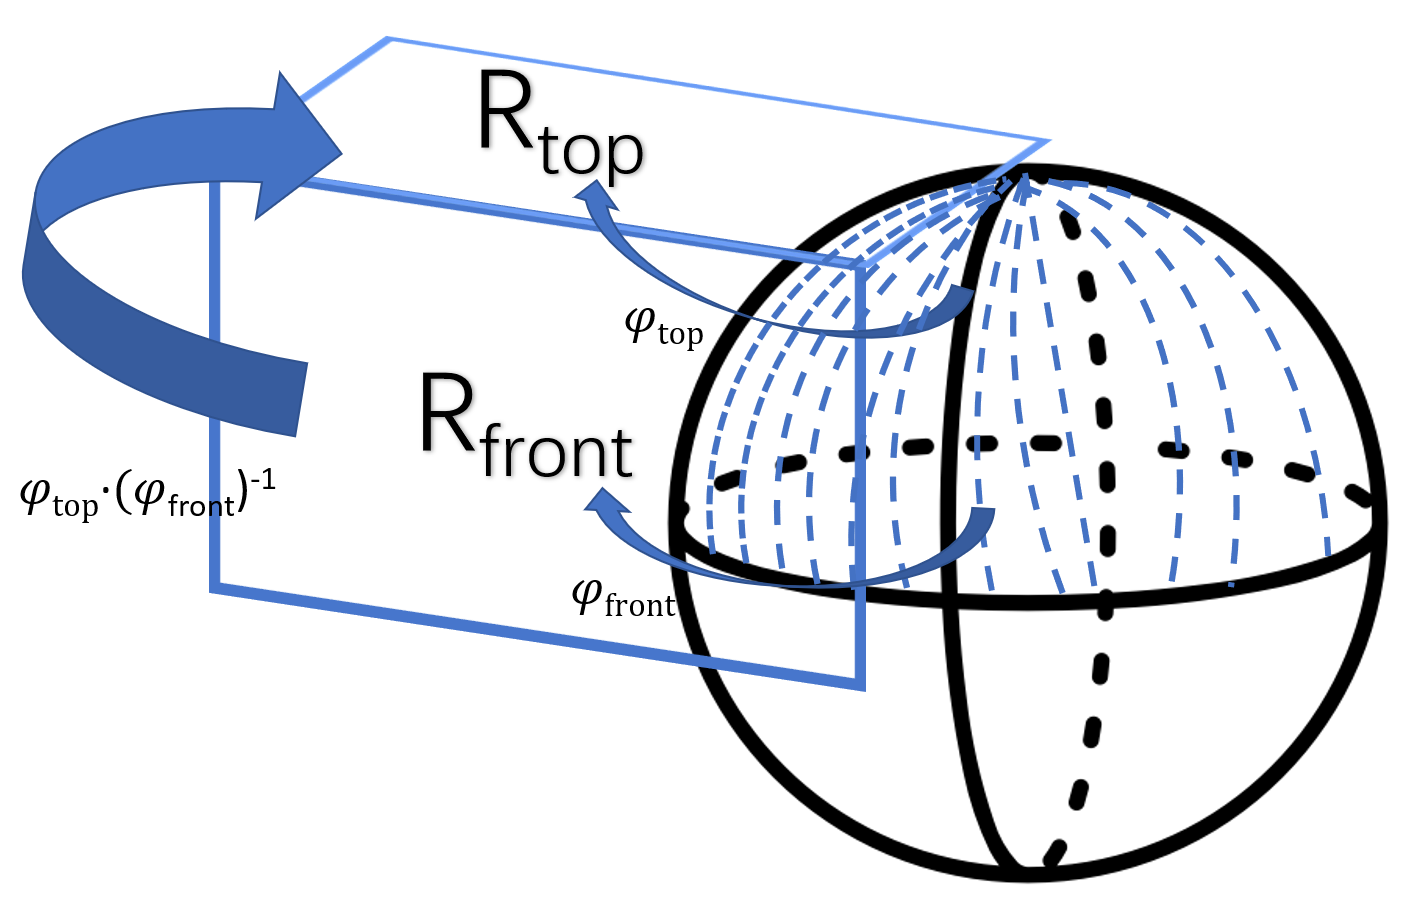
\includegraphics[width=100mm]{hemisphere.png} 
\caption{The hemisphere maps and transition map}
\end{figure}
Continuing from \textbf{Example \ref{2sphere}}, since the adjacent hemispheres have overlapping areas (intersections), it is reasonable to look at a map between the two $\mathbb{R}^2$ projections by the homeomorphisms in the intersecting region. Again, considering the "front" hemisphere with "top" as its neighbour, this is just the map from $R_{front} = \{(x,z)\ |\ x \in (-1,1), z \in (0,1)\}$ to $R_{top} = \{(x,y)\ |\ x \in (-1,1), y \in (0,1)\}$. Note that in this case the two $\mathbb{R}^2$ subspaces are identical, but it is only a coincidence. We can now consider the composition map $\varphi_{top} \circ \varphi_{front}^{-1}: R_{front} \rightarrow R_{top}$, where a point in the $R_{front}$ plane is taken back to a point on the 2-sphere by the inverse of the "front" hemisphere map, then projected onto the $R_{top}$ plane by the "top" hemisphere map. Explicitly, take $(\alpha,\beta)$ in $R_{front}$, then:\\
$\varphi_{top} \circ \varphi_{front}^{-1}(\alpha,\beta) = \varphi_{top}(\varphi_{front}^{-1}(\alpha,\beta)) = \varphi_{top}(\alpha,\sqrt{1-\alpha^2-\beta^2},\beta) = (\alpha,\sqrt{1-\alpha^2-\beta^2})$.\\
This is called a \textbf{transition map}. Figure 2 elaborates this example graphically. The proper definition of this map along with charts and atlases defined on manifolds will come later in sections 3 and 4.
\subsection{Paracompactness}
Before defining a paracompact space, we need to know what a refinement is and what it means for the refinement to be locally finite.
\begin{definition}
For a cover $C = \{U_\alpha : \alpha \in A \}$ of a topological space X, a \textbf{refinement} $D = \{V_\beta : \beta \in B \}$ of the cover $C$ is a subcover such that for all $V_\beta$ in $D$, there exists $U_\alpha $ in $C \hspace{5}$ such that $ V_\beta \subseteq U_\alpha$.
\end{definition}

\begin{definition}
An open cover $C$ of $X$ is called \textbf{locally finite} if for all $x$ in $X$, there exists $B(x)$ in $X$ where $B(x)$ is a neighbourhood of $x$ such that $B(x)$ intersects a finite number of subsets of $C$.
\end{definition}
\begin{remark}
This means that the indices of the the subsets in the open cover $C$ which intersect with the neighbourhood $B(x)$ form a finite set, that is, the set $\{\alpha \in A : U_\alpha \cap B(x) \neq \emptyset \}$ is finite.
\end{remark}

\begin{definition}
A topological space $X$ is \textbf{paracompact} if every open cover of $X$ has a locally finite open refinement.
\end{definition}
\\
\begin{remark}
Obviously, every compact space is paracompact. In a compact space every open cover has a finite subcover, where a subcover is also a refinement; and a finite refinement implies a locally finite refinement. Hence this is true by satisfying the definition.
\end{remark}

\begin{example}{}
However, a paracompact space need not to be compact as well, for instance, the Euclidean space \rn\ is clearly not compact but paracompact. \cite{paracompact}
\begin{proof}
Let $C = \{U_\alpha : \alpha \in A \}$ be a open cover of \rn. Denote $B_n(0)$ as the open ball of radius $n$ center at the origin and set $B_0 = \emptyset$. The closure of the ball $\overline{B}_n(0)$ is compact according to the Hein-Borel Theorem (as the ball clearly closed and bounded by its boundary points), therefore a finite collection of subsets in $C$ can be found to cover $\overline{B}_n(0)$ and denote it $C_n$. Now consider the set
\[
D_n = \{U \cap (\mathbb{R}^n \setminus \overline{B}_{n-1}(0))\ |\ U \in C_n\}
\]
This is a collection of open sets since the intersection of an open set with the complement of a closed set (which implies open) is also open, and each open set is a subset of an element of $C$ hence the union $D = \cup_{n = 0}^{\infty}D_n$ is an open refinement of $C$. To see that $D$ covers \rn, let \textbf{x} $\in \mathbb{R}^n$, then there exists a smallest integer $m$ such that 
\[
m-1 < ||\textbf{x}|| \leq m \leq ||\textbf{x}|| + 1
\]
Hence \textbf{x} belongs to $\overline{B}_m(0) \setminus \overline{B}_{m-1}(0)$ thus $D_m$ since $D_m$ covers $\overline{B}_m(0) \setminus \overline{B}_{m-1}(0)$. Finally $D$ is obviously locally finite since the neighbourhood $B_n(\textbf{x})$  for arbitrary \textbf{x} intersects finitely many elements in $D$, which are elements in $\cup_{i=1}^{n+m}D_i$ where $m$ is the same integer defined above.
\end{proof}
\end{example}
\section{What are Manifolds?}

Manifold is an important concept that we are going to work on. Generally speaking, a manifold is a topological space that locally resembles the Euclidean space. Before we define manifolds rigorously, we need to define what is {\bf locally Euclidean} (locally resembles Euclidean space). Locally Euclidean of dimension $n$ means that all points in this topological space have a neighbourhood that is homeomorphic (bijective and two-way continuous) to an open subset of $\mathbb{R}^n$. To be more specific, for a topological space $M$, and for each point $p\in M$, we can find a open subset $U$ of $M$ that contains $p$ and set $V$ that is an open subset of $\mathbb{R}^n$  such that there exists a homeomorphism between $U$ and $V$.\\
\\
Through the definition of locally Euclidean, we could further define charts and atlases on manifolds.
\begin{definition}
A {\bf chart} of a manifold M is a pair (U,$\varphi$) such that $\varphi$ is a homeomorphism from open subset $U$ in $M$ to an open subset U in \rn. Every point in a manifold belongs to some charts and is mapped by to some points in \rn.
\\
\end{definition}

\begin{definition}
An {\bf atlas} of a manifold is the collection of charts in a manifold M such that these charts cover M. \\
\end{definition}

There can be multiple atlases that cover a manifold. We will discuss this further when we introduce the maximal atlas.
\subsection{Topological manifold}
\begin{definition}
For a topological space $M$, we say that it is a \textbf{topological manifold} of dimension $n$ if it is: \cite{GTM}
\begin{enumerate}
    \item {\bf Hausdorff}: For every $x$ and $y$ in $M$ with $x \neq y$, there are open sets $U$ and $V$ such that $x \in U$, $y \in V$, and $U \cap V=\emptyset$.
    \item {\bf Second countable}: $M$ has a countable basis, which means there exists a countable collection $\mathbb{B}$ of open subsets of $M$ such that for any open subset $U$ of $M$ and point $p$ in $U$, there is an open set $B \in \mathbb{B}$ such that $p \in B \subset U$.
    \item {\bf Locally Euclidean}: For every point $p\in M$, there exists a neighbourhood $N$ of $p$ such that $N$ is homeomorphic to an open subset of \rn.
\end{enumerate}
\end{definition} 

\begin{figure}[tb]
\centering
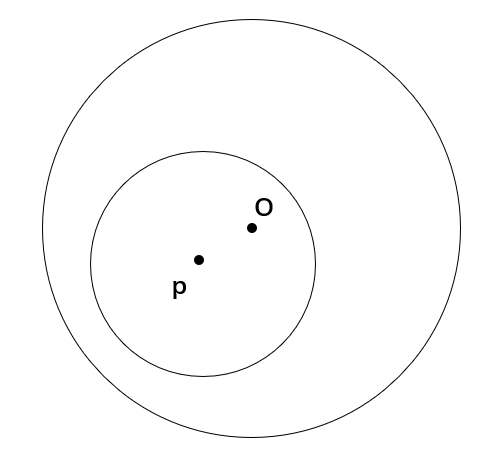
\includegraphics[width=65mm]{rational ball.png} 
\caption{rational ball}
\end{figure}
\begin{example}{(Trivial)}
The simplest topological manifold is the Euclidean space (\rn). Euclidean space is Hausdorff since it is a metric space from Analysis notes. \rn\ is also trivially locally Euclidean. Now we are left to prove that it is second-countable, and we will prove this by the rational ball approach. We define {\bf Rational balls} as open balls in \rn\ with centre of rational coordinates and rational radius.\\
\\
{\bf Claim}: The collection of rational balls in \rn\ is a basis for \rn. \cite{intro to mfds}

\begin{proof}
As shown in the figure 3, assume we have an arbitrary open set $U$ in \rn\ and arbitrary point $O\in U$. Since it is open, by definition, there exists an open ball $B(O,r)$ where $r$ is a rational number. Here we have a point $p$ with rational coordinates with $p\in B(O,r/2)$ and arbitrary point $m\in B(p,r/2)$, then since
\[
    d(O,m)\leqslant d(O,p)+d(p,m)<r/2+r/2=r
\]
we have $m\in B(O,r)$, and since $m$ is arbitrary in $B(p,r/2)$, we then have
\[
O\in B(p,r/2)\subset B(O,r)\subset U
\]
Now, since $U$ could be any open subset of $M$, we claim that the collection of rational balls is a basis for \rn, and since rational numbers are countable we could say \rn\ is second countable.
Having satisfied the three properties, \rn\ is a topological manifold.
\end{proof}

\end{example}
\\
\\
Before continuing to next examples, we look at two useful propositions that we need in proving certain topological spaces are manifolds.
\begin{proposition}
Subspace of Hausdorff space is also Hausdorff.
\begin{proof}
Assume $X$ is a Hausdorff topological space and $M$ is the subspace of $X$. Now for arbitrary distinct $a,b\in M$, since $X$ is Hausdorff, we have two open sets $U,V$ such that $a\in U$ and $b\in V$ where $M\cap U$ and $M\cap V$ are two disjoint sets that contain $a$ and $b$ respectively. Hence $M$ is also Hausdorff.
\end{proof}
\end{proposition}
\begin{proposition}
Subspace of second countable space is also second countable.
\begin{proof}
Assume $X$ is a second-countable topological space with a countable basis $\mathbb{B}$. Then for subspace $M\subset X$, $\{B\cap M\ |\ B\in \mathbb{B}\}$ is a countable basis for $M$, and therefore subspace $M$ is second-countable.
\end{proof}
\end{proposition}

Additionally, we can link these properties of topological manifolds to paracompactness.
\begin{theorem}
\label{sec para}
For a topological space $X$, if it is Hausdorff, locally Euclidean and connected, then the following statements are equivalent:\cite{harvard}
\begin{enumerate}
    \item $X$ is second-countable,
    \item $X$ is paracompact.
\end{enumerate}
\end{theorem}

\begin{corollary}
Every manifold is a paracompact space.
\begin{proof}
This is direct result from \textbf{Therorem \ref{sec para}}.
\end{proof}
\end{corollary}
\begin{figure}
\centering
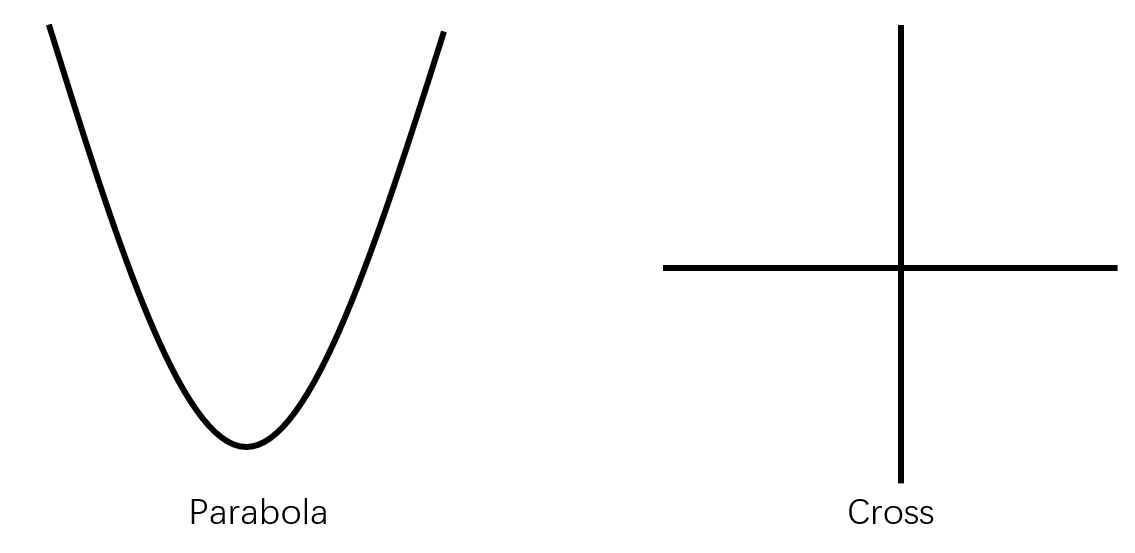
\includegraphics[width=120mm]{Parabola and Cross.png} 
\caption{ \label{overflow}}
\end{figure}
\begin{example}{(Comparison in $\mathbb{R}^2$)}We consider some simple examples in $\mathbb{R}^2$, the parabola $y=x^{2}$ and the cross shown in figure 4. They are Hausdorff and second countable since they are subspace of Euclidean space.\\
We first consider the parabola, it is locally Euclidean since we can form a homeomorphism to $\mathbb{R}$ by the map $(x,x^{2})\mapsto x$. Therefore the parabola is a topological manifold. \\
In the contrast, we could show that the cross is not a topological manifold by showing the intersection point $p$ of the two lines is not locally Euclidean. We will prove this by contradiction. If the space is locally Euclidean at $p$, there exists a neighbourhood $U$ of $p$ with a homeomorphism mapping $U$ to an open ball $B(0,\epsilon)\subset \mathbb{R}^n$ and $p$ to $0$. Now we have a new homeomorphism mapping $U\setminus \{p\}$ to $B\setminus \{0\}$, hence the number of connected components should be invariant under homeomorphism. However, $U\setminus \{p\}$ has four disjoint components while $B\setminus \{0\}$ has two components when $n=1$ and one component in other cases. Hence they are not homeomorphic and cross is not locally Euclidean hence not a smooth manifold.
\end{example}
\begin{figure}
\centering
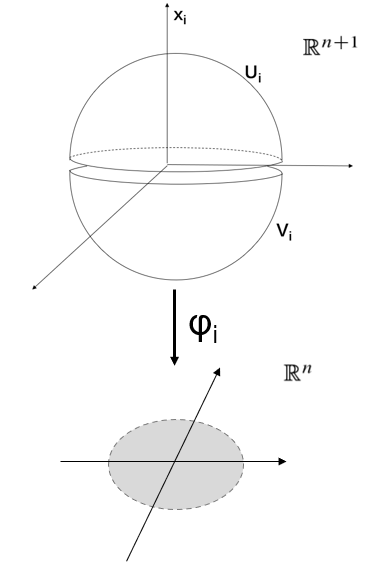
\includegraphics[width=65mm]{projection of charts of n-sphere.png} 
\caption{projection of charts of n-sphere}
\end{figure}

\begin{example}{(Sphere)}
\label{sn mfd}
Now we consider $S^n$, that is the unit $n-$sphere where $S^{n}=\{x\in \mathbb{R}^{n+1}: |x| = 1\}$. It is clearly Hausdorff and second countable being a subspace of $\mathbb{R}^{n+1}$. Then, to show spheres are topological manifolds, we need to show that they are locally Euclidean.\\
Here we could consider $(2n+2)$ charts that cover $S^{n}$ with each chart being a restriction on $S^{n}$ where $i^{th}$ coordinate being greater than or less than 0. Since $i$ could be any integer value from $1$ to $(n+1)$, there are $(2n+2)$ charts, and every point $p$ belongs to one of the charts. For each chart with $i^{th}$ coordinate being restricted, we could define a homeomorphism from $S^{n}$ to \rn\ by omitting the $i^{th}$ coordinate.\\
Formally, we express points on the sphere by Cartesian coordinates with $(n+1)$ coordinates as $(x_1,…,x_{n+1})$. Then, as shown in figure 5, we denote the $(2n+2)$ charts by $U_1,…,U_n,U_{n+1},V_1,…
\\
,V_n,V_{n+1}$ where $U_i=\{(x_1,…,x_{n+1})\in S^n:x_i>0\}$ and $V_i=\{(x_1,…,x_{n+1})\in S^n:x_i<0\}$ with the map from $S^n$ to \rn\ as  $\varphi_i(x_1,…,x_{n+1})=(…,x_{i-1},x_{i+1},…)$ for $U_i$ and $V_i$. This map is a continuous projection from $\mathbb{R}^{n+1}$ to \rn. The continuous inverse map is defined by $\varphi^{-1}(…,x_{i-1},x_{i+1},…)=(x_1,…,x_i,…,x_{n+1})$ where $x_i=(1-\sum_{j\neq i}{x_j}^2)^{1/2}$. Hence it is a homeomorphism. Sphere is an important kind of manifolds that we will continue to discuss it later.
\end{example}

\subsection{Differentiability and Smoothness}
In order to make use of manifolds and allow as to do calculus (for example, use integration to calculate volume and use differentiation to determine curvatures) on them, we will have to introduce smooth manifolds and differentiable manifolds. But before doing so, we need to know some basic definitions related to differentiability and smoothness. For a map from one Euclidean space to another Euclidean space, we are familiar with definition of differentiability in this situation as having continuous partial derivatives from Analysis notes on differentiation in higher dimensions. We now introduce a notation $C^{k}$ which denotes the class of functions where their $k^{th}$ derivatives are continuous. For instance, a continuous function is $C^{0}$. A smooth map (or function) is defined as having continuous derivative of infinite order, and therefore a smooth map is $C^{\infty}$. How do we relate these definitions to a map between other topological manifolds rather than just Euclidean spaces? This is where we need to define an analytic structure. But before doing so, let's first make a remark on homeomorphism that important properties including differentiability and smoothness is not invariant under homeomorphism. We could consider a very simple example. Looking at the figure 6 from circle to square, it is a trivial homeomorphism by considering the function with respect to angle $\theta$. However the function has a derivative and is differentiable in the boundary of circle but clearly not when it comes to the four corners in the boundary of square. Therefore, we could conclude that differentiability is not invariant under homeomorphism. In fact, there is a special type of homeomorphism we defined before that the property of differentiaility and smoothness can be invariant, and this type of homeomorphism is diffeomorphism. We will further elaborate on it when we define the smooth manifold.
\begin{figure}[tb]
\centering
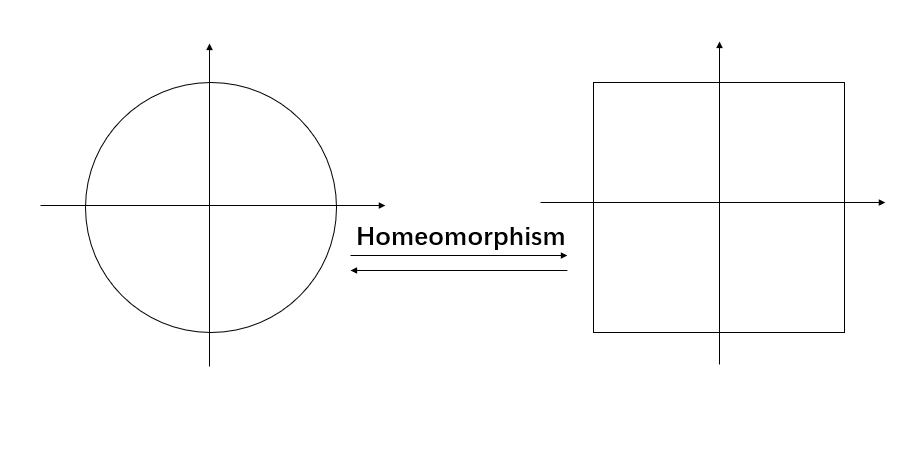
\includegraphics[width=100mm]{circle versus square.png} 
\caption{circle to square}
\end{figure}
Now we need to introduce the concept {\bf transition map} before we can finally define differentiable and smooth atlas to properly state differentiable and smooth manifolds respectively.
\\
\begin{definition}
For two charts $(U,\varphi)$ and $(V,\psi)$ in a topological manifold, we say if U and V are not disjoint then the composition map $\varphi$$\circ$$\psi ^ {-1}:\psi(U\cap V)\rightarrow \varphi(U\cap V)$, or $\psi$$\circ$$\varphi ^ {-1}:\varphi(U\cap V)\mapsto \psi(U\cap V)$ defined on the intersection of U and V is a \textbf{transition map}.
\end{definition}
\\
\begin{figure}[tb]
\centering
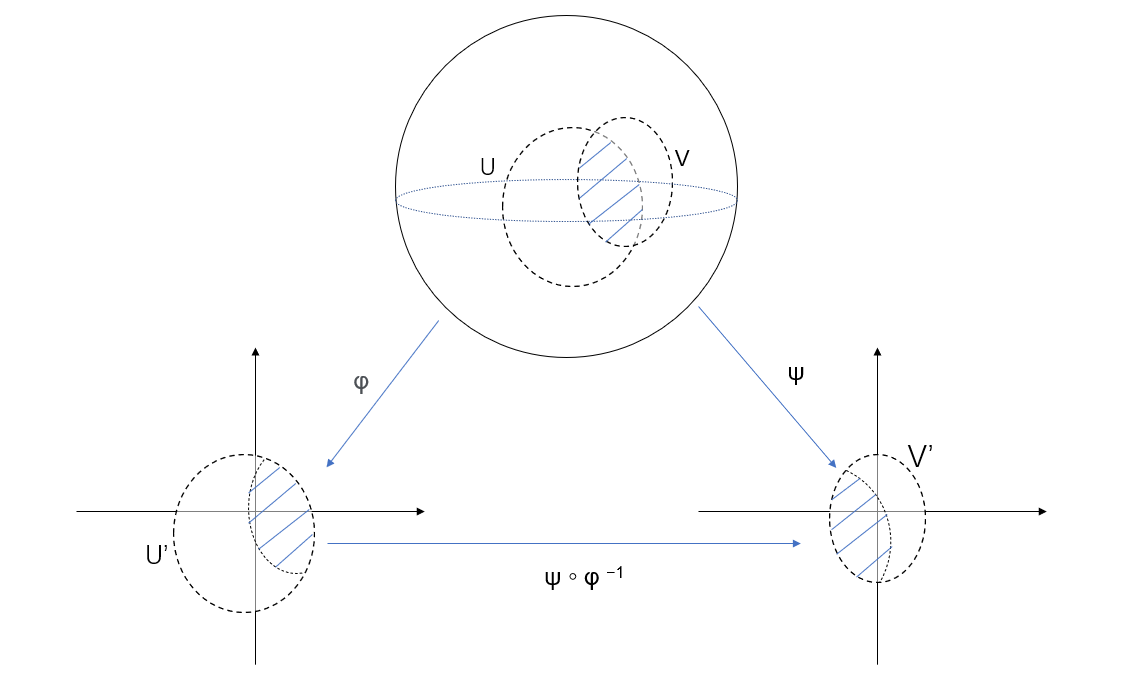
\includegraphics[width=160mm]{transition map.png} 
\caption{transition map}
\end{figure}
An example of transition map is shown in figure 7 named 'transition map'. We have a sphere $S^2$ in $\mathbb{R}^3$ with two charts $(U,\varphi)$ and $(V,\psi)$. $U$ maps to $U'$ on $\mathbb{R}^2$ and $V$ maps to $V'$ on $\mathbb{R}^2$ as shown in the diagram. We can see that the transition map $\psi$$\circ$$\varphi ^ {-1}$ maps $\varphi(U\cap V)$ to $\psi(U\cap V)$ exactly as the definition.

\subsection{Differentiable Manifolds}
Since we have already defined transition maps between charts, we could now define the differentiable structure on topological manifolds by providing a differentiable atlas, and here is how we define differentiable atlas by transition maps.
\begin{definition}
An atlas $\mathbb{A}$ is called a {\bf differentiable atlas} if any two charts $(U,\varphi)$ and $(V,\psi)$ in $\mathbb{A}$ are either disjoint or their transition map $\psi$$\circ$$\varphi ^ {-1}$(and its inverse) is differentiable ($C^{k}$, where $k\neq 0$). \\
\end{definition}
However, as we have mentioned before, we want to define a differentiable ($C^{k}$) structure on a given topological manifold $M$ by a differentiable atlas and define a differentiable function $f:M\rightarrow \mathbb{R}$ such that $f\circ \varphi^{-1}$ is differentiable for all charts $(U,\varphi)$ in the atlas. Under many circumstances, there will be more than one choice of atlas that result in the same differentiable structure where the same collection of differentiable functions are determined on the topological manifold. Therefore, we need to introduce the {\bf maximal differentiable atlas} as the differentiable atlas that is not contained in any larger differentiable atlas.

We are now able to conclude the section by defining the differentiable manifolds.
\begin{definition}
A {\bf differentiable manifold} is a pair $(M,\mathbb{A})$ where $\mathbb{A}$ is a maximal differentiable atlas on a topological manifold $M$.
\end{definition}
\subsection{Smooth Manifolds}
Smooth manifolds are an important kind of manifolds that we explore when we go through Lie groups and homogeneous spaces. Since we have already defined differentiable manifolds, the definition of smooth manifolds follows easily. In general, smooth manifolds are a special class of $C^{k}$ manifolds when we take $k$ as $\infty$. Here we follows the same way and define smooth manifolds again by introducing some alternative expressions. We say two charts $(U,\varphi)$ and $(V,\psi)$ are {\bf smoothly compatible} if either they are disjoint or their transition map is a diffeomorphism. Then we could define smooth atlas.

\begin{definition}
An atlas is a {\bf smooth atlas} if every chart of it is smoothly compatible with each other.
\end{definition}
Note that in smooth manifolds, we also need a maximal smooth atlas defined in the same way as maximal atlas in differentiable manifolds. So to conclude:
\begin{definition}
A {\bf smooth manifold} is a pair $(M,\mathbb{A})$ where $\mathbb{A}$ is a maximal smooth atlas on a topological manifold $M$.
\end{definition}
As usual, we will provide some examples of smooth manifolds.
\begin{example}

\rn\ is a smooth manifold. This is trivial if we consider the smooth structure with single chart $(\mathbb{R}^{n},id)$. Here we also consider a simple case why we need maximal smooth atlas. Consider two atlas $(\mathbb{R}^{n},id)$ and $(B(r),id)$ where $B(r)$ stands for the collection of rational balls we defined earlier. Both atlas covers \rn\ and defines identical smooth structure. In this case, we use the maximal atlas $(\mathbb{R}^{n},id)$.
\end{example}

\begin{example}
$S^n$ is a smooth manifold. As we have shown that $S^n$ is a manifold in \textbf{Example \ref{sn mfd}}, if we use the same atlas it is trivial to see that the transition map is smooth.
\end{example}

\begin{example}

$GL_n(\mathbb{R})$ is also a smooth manifold. This is not so trivial.
\end{example}
Before proving \textbf{Example 3.13}, there are several propositions needed to be shown. Consider arbitrary $n\times n$ matrices, we know $\mathbb{R}^{n^2}$ is smooth. Now consider the determinant map is $\det:\mathbb{R}^{n^2} \rightarrow \mathbb{R}$.
\begin{proposition}
\label{detmap}
The determinant map is a continuous map.
\begin{proof}
For arbitrary matrices $A=(a_{ij})_{n\times n}$, $B=(b_{ij})_{n\times n}$,
$\det(A) = \sum_{\sigma \in S_{n}} sgn(\sigma) \Pi_{i=1}^{n}a_{i,\sigma _{i}}$, $\det(B) = \sum_{\sigma \in S_{n}} sgn(\sigma) \Pi_{i=1}^{n}b_{i,\sigma _{i}}$, where $S_{n}$ is the set of all permutations of ${1,2,...,n}$, and $\sigma(i)=\sigma_{i}$.
\\
Define $m = max_{1\leqslant i, j\leqslant n}\{|a_{ij}|,\ |b_{ij}|\}$, then 
\begin{align}
    |\det(A)- \det(B)| &=|\sum_{\sigma \in S_{n}}sgn(\sigma)(\Pi_{i=1}^{n}a_{i,\sigma _{i}}-\Pi_{i=1}^{n}b_{i,\sigma _{i}})|
    \\
    (by\ triangle\ inequality) &\leqslant \sum_{\sigma \in S_{n} }|\Pi_{i=1}^{n}a_{i,\sigma _{i}}-\Pi_{i=1}^{n}b_{i,\sigma _{i}}| 
    \\
    & = \sum |a_{1,\sigma_{1}}\cdot a_{2,\sigma_{2}}\cdot ...\cdot a_{n,\sigma_{n}} - b_{1,\sigma_{1}}\cdot b_{2,\sigma_{2}}\cdot ...\cdot b_{n,\sigma_{n}}|
    \\
    & = |(a_{1,\sigma_{1}}-b_{1,\sigma_{1}})a_{2,\sigma_{2}}a_{3,\sigma_{3}}\cdot \cdot \cdot a_{n,\sigma_{n}}
    \\
    &+b_{1,\sigma_{1}}(a_{2,\sigma_{2}}-b_{2,\sigma_{2}})a_{3,\sigma_{3}}a_{4,\sigma_{4}}\cdot \cdot \cdot a_{n,\sigma_{n}}+\cdot \cdot \cdot
    \\
    &+b_{1,\sigma_{1}}b_{2,\sigma_{2}}\cdot \cdot \cdot(a_{n,\sigma_{n}}-b_{n,\sigma_{n}})|
    \\
    & \leqslant \sum_{\sigma \in S_{n}}\sum_{i=1}^{n}(m^{n-1}\cdot |a_{i,\sigma_{i}}-b_{i,\sigma_{i}}|)
\end{align}
Now we can use the $\epsilon - \delta$ approach:\\
%\begin{proof}\label{$\epsilon - \delta$ proof}
For all $\epsilon > 0$, set $\delta > 0$ such that $\delta = \frac{\epsilon}{2m^{n-1}\cdot n \cdot n!}$. If $\parallel A-B \parallel\ <\ \delta$, then $\parallel a_{ij}-b_{ij} \parallel \ <\ \delta,\ \forall 1 \leqslant i, j\leqslant n$, hence
\begin{align}
&\parallel \det(A)-\det(B)\parallel\ \leqslant\ \sum_{\sigma \in S_{n}}\sum_{i=1}^{n}(m^{n-1}\cdot |a_{i,\sigma_{i}}-b_{i,\sigma_{i}}|)
\\
&\leqslant n!\cdot n \cdot m^{n-1}\cdot \delta = \frac{\epsilon}{2} < {\epsilon}
\end{align}
And this proves the determinant map is continuous.
\end{proof}
\end{proposition}
\\
$GL_{n}(\mathbb{R})$ is defined on the set of $n\times n$ invertible matices with a group operation of ordinary matrix multiplication. We know from first year that a matrix $A$ is invertible $\Leftrightarrow$ $\det(A)\ \neq\ 0$.\\
So we can say: $GL_{n}(\mathbb{R})\ :=\ \{ A\in \mathbb{R}^{n^{2}}\ |\ \det(A)\ \neq\ 0\}$. (That is $GL_{n}(\mathbb{R})\ \subset\ \mathbb{R}^{n^{2}}$)
%\end{proof}
\begin{proposition}
$GL_{n}(\mathbb{R})$ is open in $\mathbb{R}^{n^{2}}$.
\begin{proof}
Consider the complement of $GL_{n}(\mathbb{R})$, which is the set of matrices with determinant 0. Since $\{0\}$ is a closed set in \rn, and for the continuous determinant map ($\mathbb{R}^{n^{2}}\rightarrow \mathbb{R}$), the pre-image of a closed set is also closed. Hence the complement of a closed set is open, in another words, $GL_{n}(\mathbb{R})$ is an open subset of $\mathbb{R}^{n^{2}}$.
\end{proof}
\end{proposition}
As $\mathbb{R}^{n}$ is a trivial smooth manifold, we conclude that $\mathbb{R}^{n^{2}}$ is also a smooth manifold. We now want to show that $GL_{n}(\mathbb{R})$ is a manifold as well.
\begin{proposition}
$GL_{n}(\mathbb{R})$ is a manifold.
\begin{proof}
Let $\{(U_{\alpha},\phi_{\alpha})\}$ be an atlas for $\mathbb{R}^{n^{2}}$.\\
Then, $\{(U_{\alpha} \cap GL_n(\mathbb{R}),\psi_{\alpha})\}$ where $\psi: U_{\alpha} \cap GL_{n}(\mathbb{R}) \rightarrow \mathbb{R}^{n^{2}}$ is constructed by restricting $\phi_{\alpha}$ to only cover $\psi: U_{\alpha} \cap GL_{n}(\mathbb{R})$. This forms an atlas for $GL_{n}(\mathbb{R})$, hence $GL_{n}(\mathbb{R})$ is a manifold.
\end{proof}
\end{proposition}
Another proof is to consider the determinant function. For $A\in GL_{n}(\mathbb{R})$, $\det(A) = \sum_{\sigma \in S_{n}} sgn(\sigma) \Pi_{i=1}^{n}a_{i,\sigma _{i}}$. This is a polynominal expression in $a_{ij}$, so the map $\det:\ \mathbb{R}^{n^{2}}\rightarrow \mathbb{R}$ is infinitely differentible. (that is to say determinant is a smooth map.). We can then represent $GL_{n}(\mathbb{R})$ as the pre-image of the determinant map: $GL_{n}(\mathbb{R})\ =\ \det^{-1}(\mathbb{R}\setminus\{0\})$. Applying the implicit function theorem, we obtain that $GL_{n}(\mathbb{R})$ is a manifold.\\
Now we further show the smoothness of two matrix operations.
\begin{proposition}
Matrix multiplication is a smooth map.
\begin{proof}
Breaking down the matrix multiplication into $(AB)_{ij}=\sum_{k=1}^n A_{ik}B_{kj}$. This is a polynomial expression, here matrix multiplication is smooth.
\end{proof}
\end{proposition}
\begin{proposition}
Taking the inverse of a matrix is a smooth map.\\ 
\begin{proof}
We know (by Cramer's rule) that  $A^{-1}=\dfrac{\mbox{adj}(A)}{\det(A)}$, this is a polynomial divided by another polynomial. Hence it is smooth if $det(A)\neq 0$.
\end{proof}
\end{proposition}
Combining the two propositions above gives that $GL_{n}(\mathbb{R})$ is a smooth manifold (this may not seem to be a direct result, but we will show why this works very shortly). It turns out that this result implies that $GL_{n}(\mathbb{R})$ is a also lie group, which is a group relating to manifolds that we are about to discuss in the next section.\\

\section{Lie groups and actions on Manifolds}
In this section we will start with definitions on some properties of group actions. \cite{gp action wiki}
\begin{definition}
\textbf{Free}: For a group G acting on X, the action is free if the only element that has fixed points is the identity. So free group actions on non-empty sets are always faithful.
\end{definition}

\begin{definition}
\textbf{Proper}: For a map to be proper is when the pre-image of a compact set is compact. A group(G) action on X is proper when the map $G \times X\rightarrow X\times X$ : $(g,x) \mapsto (g\cdot x,x)$ is proper.
\end{definition}

\begin{definition}
\textbf{Transitive} if there exist only one orbit.
\end{definition}

\begin{definition}
\textbf{Lie group}\cite{rie geo} is a group $G$ that is also a smooth manifold and the map $G \rightarrow G$, $(g,h)\mapsto gh^{-1}$, with $g,h\in G$ is smooth.
\end{definition}
As the composition of smooth functions is also smooth, proving that taking the inverse and applying the group operations to all elements in G are smooth is sufficient to prove the smooth map property.

\begin{definition}
A \textbf{submanifold} is a subset of a manifold that is locally Euclidean.
\end{definition}

\begin{theorem}{(\textbf{E.Cartan's closed-subgroup theorem}):} \cite{cartan subgroup}
\label{Ecartan}
Any closed subgroup H of a lie group G is a lie subgroup (and hence a submanifold) of G.
\end{theorem}
We now want to define a special group representing matrices with constraints on the determinant and derive some results about it.
\begin{definition}
The \textbf{special linear group} $SL_{n}(\mathbb{R})$ is the set of $n\times n$ invertible matrices with determinant 1 and with the standard matrix multiplication as the group operation.
\end{definition}
\begin{proposition}
$SL_{n}(\mathbb{R})$ is a subgroup of $GL_{n}(\mathbb{R})$.
\begin{proof}
Conduct the subgroup test. $\det(I_{n})=1$, hence $SL_{n}(\mathbb{R})$ is a non-empty subset of $GL_{n}(\mathbb{R})$.
Let A, B be arbitrary matrices $\in SL_{n}(\mathbb{R})$. Then A, B are invertible, with $\det(A) =\det(B)=1$. As B is invertible, $B^{-1}$ exists and $\det(B^{-1})=1$. Since $\det(AB^{-1})= \det(A)\times \det(B^{-1})=1$, $AB^{-1}\in\ SL_{n}(\mathbb{R})$. By subgroup test, we have shown $SL_{n}(\mathbb{R}) \leqslant GL_{n}(\mathbb{R}) $. As $SL_{n}(\mathbb{R}) \leqslant GL_{n}(\mathbb{R})$, we also know $SL_{n}(\mathbb{R})$ is closed algebraically in $GL_{n}(\mathbb{R})$.
\end{proof}
\end{proposition}

\begin{proposition}
\label{SLnclosed}
$SL_{n}(\mathbb{R})$ is a closed subgroup of $GL_{n}(\mathbb{R})$.
\end{proposition}
before the proof we need to define two terms.
\begin{definition}
A subgroup $H$ is called \textbf{topologically closed} in a group if $H$ contains all its limit points.
\end{definition}

\begin{definition}
A $n\times n$ matrix is called \textbf{singular} if it has determinant 0.
\end{definition}

\begin{proof}
In the context of the subgroup $SL_{n}(\mathbb{R})$ of the group $GL_{n}(\mathbb{R})$, to claim that $SL_{n}(\mathbb{R})$ is a topologically closed subgroup of $GL_{n}(\mathbb{R})$, we will need to prove $SL_{n}(\mathbb{R})$ contains all non-singular limit points. (singular ones aren't even in $GL_{n}(\mathbb{R})$)\\
We showed that $\det:\ GL_{n}(\mathbb{R})\ \rightarrow\ \mathbb{R}\setminus \{0\}$ is continuous in \textbf{Proposition \ref{detmap}}, and $SL_{n}(\mathbb{R})$ can also be written as $\det^{-1}\{1\}$. As $\{1\}$ is closed in $\mathbb{R}$, the pre-image $SL_{n}(\mathbb{R})$ is also closed in $GL_{n}(\mathbb{R})$.
\end{proof}

By \textbf{Proposition \ref{SLnclosed}}, we have shown that $SL_{n}(\mathbb{R})$ is a topologically closed subgroup of the lie group $GL_{n}(\mathbb{R})$. Apply E.Cartan's closed-subgroup theorem, $SL_{n}(\mathbb{R})$ is also a lie group and thus a submanifold of $GL_{n}(\mathbb{R})$. Thus, by definition of manifold and submanifold, $SL_{n}(\mathbb{R})$ is a manifold.

\begin{definition}
The \textbf{special orthogonal group} $SO_{n}(\mathbb{R})$ is the set of $n\times n$ invertible matrices $Q$ satisfying:
\begin{enumerate}
    \item $\det(Q)=1$
    \item $QQ^{\mathbf{\top}} = I$
\end{enumerate}
\end{definition}

\begin{proposition}
$SO_{n}(\mathbb{R})\ \leqslant\ SL_{n}(\mathbb{R})$
\end{proposition}
\begin{proof}
It is obvious that $SO_n(\mathbb{R})$ is a subset of $SL_n(\mathbb{R})$. Therefore, again, we conduct the subgroup test. Trivially $I_n \in SO_n(\mathbb{R})$ since $\det(I_n)=1$ and $I_n = I_n^{\top}$, hence $SO_n(\mathbb{R})$ is non-empty. Let $P,\  Q$ be arbitrary matrices in $SO_n(\mathbb{R})$, then $\det(P)=\det(Q)=1,\ PP^{\top}=QQ^{\top} = I_n$. Consider the matrix $PQ^{-1}$, then
\begin{gather*}
\det(PQ^{-1}) = \det(P)\det(Q^{-1}) = \det(P)\det(Q)^{-1} = 1\\
PQ^{-1}(PQ^{-1})^{\top} = PQ^{-1}(Q^{-1})^{\top}P^{\top} = PQ^{-1}(Q^{\top})^{-1}P^{\top} = P(QQ^{\top})^{-1}P^{\top} = PI_nP^{\top} = I_n
\end{gather*}
Hence $PQ^{-1} \in SO_n(\mathbb{R})$, which implies that $SO_n(\mathbb{R})$ is a subgroup of $SL_n(\mathbb{R})$.
\end{proof}

\begin{proposition}
$SO_{n}(\mathbb{R})$ is a topologically closed subgroup of $SL_{n}(\mathbb{R})$.
\begin{proof}
Firstly we want to consider the tranpose map $T:\mathbb{R}^{n^2} \rightarrow \mathbb{R}^{n^2},\ T(A) = A^{\top}$.
\begin{claim}
$T$ is a continuous map.
\begin{claimproof}
For arbitrary matrices $A=(a_{ij})_{n\times n},\ B=(b_{ij})_{n\times n}$, we have $A^{\top} = (a_{ji})_{n \times n},\ B^{\top} = (b_{ji})_{n \times n}$. Then use the $\epsilon-\delta$ approach, $\forall \epsilon > 0$, set $\delta = \epsilon$. If $\parallel A-B \parallel\ <\ \delta$, then $\parallel a_{ij}-b_{ij} \parallel \ <\ \delta,\ \forall 1 \leqslant i, j\leqslant n$, hence $\parallel a_{ji}-b_{ji} \parallel \ <\ \delta = \epsilon\  \Rightarrow\  \parallel A^{\top}-B^{\top} \parallel\ <\ \epsilon$
\end{claimproof}
\end{claim}\\
It is known that matrix multiplication is a continuous map, hence the map $\mathbb{R}^{n^2} \rightarrow \mathbb{R}^{n^2},\ A \mapsto AA^{\top}$ is just the composition of two continuous maps, which is also continuous. Consider the continuous map $O:SL_n(\mathbb{R}) \rightarrow SL_n(\mathbb{R}),\ O(A) = AA^{\top}$ (this is valid as the map preserves the determinant 1), then $SO_n(\mathbb{R})$ is the pre-image $O^{-1}(\{I_n\})$. As $\{I_n\}$ is closed in $SL_n(\mathbb{R})$, the pre-image $SO_n(\mathbb{R})$ is also closed.
\end{proof}
\end{proposition}

By a similar argument, we can use E.Cartan's closed-subgroup theorem to show that $SO_{n}(\mathbb{R})$ is also a Lie group and a submanifold of $SL_{n}(\mathbb{R})$.\\
\textbf{Conclusion:} $GL_{n}(\mathbb{R}),\ SL_{n}(\mathbb{R}),\ SO_{n}(\mathbb{R})$ being both lie groups and manifolds implies that they are smooth manifolds with the smooth map of matrix multiplication.
\\

\section{Homogenous spaces}

\begin{definition}
An \textbf{isotropy group}\cite{Rowland} $G_{x}$ is a subgroup of G, which for all $g$ in $G_{x},\ g\cdot x=x$.
\end{definition}

\begin{example}
$SO(n)$ is the isotropy group of $SO(n+1)$. (we will use $SO(n)$ to denote $SO_n(\mathbb{R})$ now for convenience)\cite{Rowland}
\begin{proof}
Point $e_{1}=(1,0,...,0)$ on $SO(n+1)$ gives a subspace of dimension $n$, that is $\{e_{2},\ e_{3},\ ...
,\ e_{n+1}\}$, this forms a basis of the isotropy group. Note that the group acts transitively, hence all the isotropy groups given arbitrary points are isomorphic to this isotropy group, which is $SO(n)$.
\end{proof}
\end{example}
\\

\begin{definition}
\textbf{Homogeneous space:} A homogeneous space for a group G can be a smooth manifold, or in general a topological space X on which G acts transitively.
\end{definition}

Examples of homogeneous space will be projective space, hyperbolic spaces, affine spaces etc.
\begin{remark}
\textbf{Projective space}\cite{upenn}: Defined on a vector space $V$ over a field $F$, the projective space $P(V)$ is a collection of equivalence class of $V$ defined as $x\sim y$ if $x= \lambda y$, with $\lambda \in F$.\\
\textbf{Hyperbolic space}: Homogeneous space with a constant negative curvature.
\end{remark}

\begin{example}

The n-sphere $(S^{n})$ is a homogeneous space.
\begin{proof}
Consider $SO(n+1)$ as the lie group, and $SO(n)$ is the isotropy subgroup of $SO(n+1)$.\\
To prove $S^{n}$ is a homogeneous space, we need to prove is that $S^{n}$ is a smooth manifold, a lie group action $SO(n+1)$ acted on $S^{n}$, and that $SO(n+1)$ acts transitively. We have already shown that $S^n$ is a smooth manifold and $SO(n)$ is a lie group, therefore what is left to do is to prove $SO(n+1)$ acts transitively.\\
Given an arbitrary point $x$ on the n-sphere, it's obvious that given any $g$ in $SO(n+1)$, $g\cdot x \in\ S^{n}$, since orthogonal matrix preserves the length of the vector.\\
Note that $S^{n}$ is diffeomorphic to $SO(n+1)/SO(n)$, and $SO(n)$ is the isotropy group of $SO(n+1)$.
\end{proof}
\end{example}
\\


\section{Fiber bundles}

\begin{definition}
For $E$ (total space), $B$ (base fiber), $F$ (fiber) topological spaces and a continuous map $\pi : E \rightarrow B$ form a \textbf{fiber bundle with fiber F} \cite{fiber bundle} if:
\begin{enumerate}
    \item B is a connected topological space.
    \item The natural projection map $\pi: E \rightarrow B$ is surjective.
    \item Each element in the base fiber has an open neighbourhood contained within the base fiber. That is for all $x \in B$, $\exists$ open neighbourhood $U_{x} \subset B$ \cite{Lawn}    
    \item There exists a homeomorphism $\varphi: \pi^{-1}(U_{x})\rightarrow U_{x}\times F$, that is a topological isomorphism.
\end{enumerate}
\end{definition}

\begin{remark}
A rank $r$ vector bundle is called \textbf{trivial} with the associated map $\pi: E \rightarrow B$, if it is not isomorphic to the trivial bundle $B\times R^{r}$. 
\end{remark}
\\
\begin{figure}[tb]
\centering
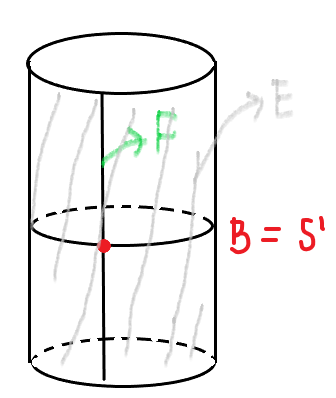
\includegraphics[width=40mm]{fiber bundle.png} 
\caption{ \label{overflow}}
\end{figure}
\\
\textbf{Trivial bundle}: An example is shown in figure 8. Imagine that the cylinder has infinite height (in both directions), then it is a trivial bundle. Firstly, this is a fiber bundle with total space as the surface of the cylinder; base space as $S^{1}$, the middle circle; fiber space as the points (red dot) on the base and extended to both directions as shown in the graph. It is clear that for any point on the surface of the cylinder, it can be represented as a product coordinate $(b,f)$, with $b$ in $B$, $f$ in $F$. The projective map is from $(b,f)$ to $b$. And by definition, this is clearly a trivial bundle.

\textbf{Non-trivial bundle}: Mobiüs strip and klein bottle. Think of mobiüs strip as a twisted circle cross fibers, then it couldn't be trivial with the same reason as the klein bottle.

\newcommand{\iso}{\xrightarrow{
   \,\smash{\raisebox{-0.65ex}{\ensuremath{\scriptstyle\sim}}}\,}}
\begin{definition}
\textbf{Principal bundles}: A \textbf{principal G-bundle}\cite{Lawn} with a topological space G, is a fiber bundle $\pi:\ E\rightarrow B$, together with a continuous right action $\omega: E\times G \rightarrow E$, and that $\tilde{\pi}:= E\times G \xrightarrow{\mu} E \xrightarrow{\pi} B$ and $E\times G \xrightarrow{\pi \times C} B \times \{e \} \iso B$ commutes with the map $C$, a map from everything to identity. And given a point $x\in B$, $G$ acts freely and transitively on the fiber $F_{x}$.
\end{definition} 

In general, both homogeneous spaces and principal bundles have transitive group actions, but in homogeneous space case, it is a group (usually a lie group) acting on the space, while in principal bundle it is the group $G$ acting on fibers which then gives back another point on the same fiber.\\
But if we see the isotropy groups as fibers, lie group/isotropy group as the base space, then a homogeneous space could be diffeomorphic to the quotient space.

%  \unsure{Ex: Is this correct?}
% homogenous space as fiber bundle here

\begin{figure}[tb]
\centering
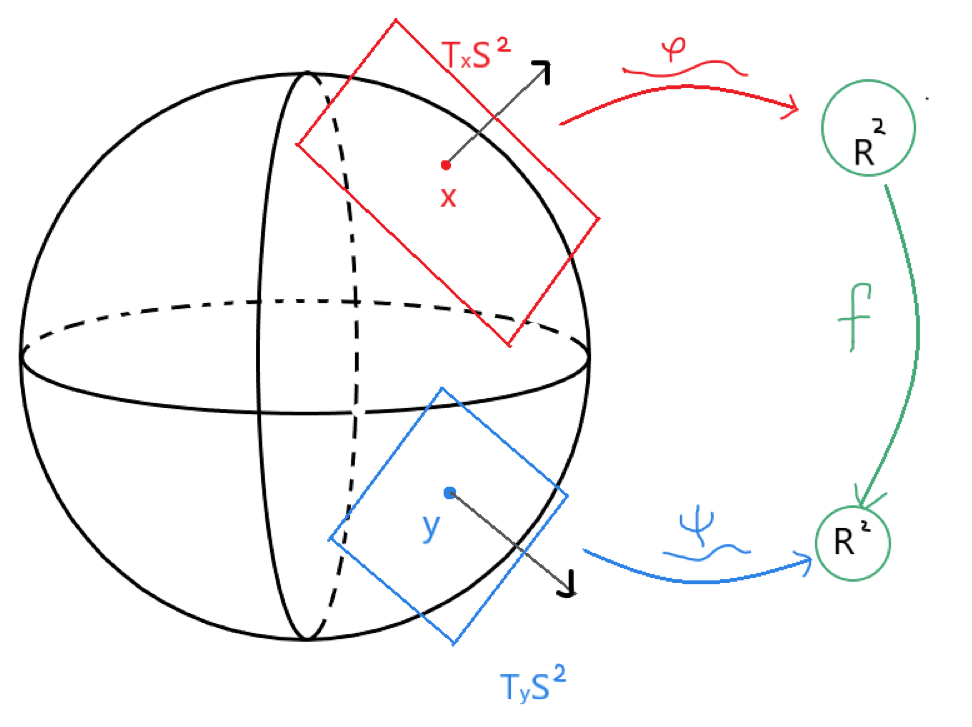
\includegraphics[width=110mm]{tangent to R.png} 
\caption{ \label{overflow}}
\end{figure}


\section{Applications of homogenous spaces}

According to Section 5, a homogenous space constructed in this way is diffeomorphic to the cross product of the quotient ring G over the isotropy group and the isotropy group itself. This cross product is just the original group G, and therefore the homogenous space behaves like a principal fiber bundle. We could not go into further detail as this was outside the scope of our project. 
However, this is an important result that allows us to form 'connections' and move 'across tangent spaces' of manifolds, as shown in figure 9. \cite{geom homog}

In more applied mathematics, we can prove certain results that are used in mathematical gauge theory.

\begin{thebibliography}{999}
\bibitem{columbia}
Tu.  \textit{Group acting on sets}. Available from:
\url{http://www.math.columbia.edu/~rf/groupactions.pdf}[Accessed from 14th June 2021]

\bibitem{einstein mfd}
Arthur L. Besse. \textit{Einstein Manifolds}. Germany: Springer-Verlag Berlin Heidelberg New York; 1987. p.179-180

\bibitem{paracompact}
Tyrone Cutler. \textit{Paracompact Spaces}. Available from: \url{https://www.math.uni-bielefeld.de/~tcutler/pdf/Paracompact\%20Spaces.pdf}[Accessed from 14th June 2021]

\bibitem{harvard}
Hiro Lee Tanaka. \textit{Second countability and Paracompactness}. Available from: \url{http://people.math.harvard.edu/~hirolee/pdfs/2014-fall-230a-lecture-02-addendum.pdf}[Accessed from 14th June 2021]

\bibitem{gp action wiki}
Zuoqin Wang. \textit{Proper actions and Orbit spaces}.[Lecture] University of Science and Technology of China.5th November 2013

\bibitem{cartan subgroup}
Zuoqin Wang. \textit{Cartan’s Closed Subgroup Theorem}[Lecture]  University of Science and Technology of China.18th October 2013

\bibitem{Rowland}
Todd Rowland. \textit{Isotropy group}. Available from: \url{https://mathworld.wolfram.com/IsotropyGroup.html}[Accessed from 14th June 2021]

\bibitem{upenn}
University of Pennsylvania. \textit{Chapter 5, Basics of Projective Geometry}. Available from \url{https://www.cis.upenn.edu/~jean/gma-v2-chap5.pdf}[Accessed from 14th June 2021]

\bibitem{fiber bundle}
XylyXylyX. \textit{What is a Manifold? Lesson 12: Fiber Bundles - Formal Description} [video] 2016. Available from: \url{https://www.youtube.com/watch?v=AUVG2ghNfic}[Accessed from 14th June 2021]

\bibitem{rie geo}
Sylvestre Gallot, Dominique Hulin, Jacques Lafontaine \textit{Riemannian Geometry} Chapter 1: DIFFERENTIAL MANIFOLDS, Germany: Springer-Verlag Berlin Heidelberg; 1987

\bibitem{intro to mfds}
Tu L.W. \textit{An introduction to manifolds} Springer; 2008

\bibitem{GTM}
John M. Lee \textit{Introduction to smooth manifolds} Springer; 2006

\bibitem{Lawn}
Marie-Amelie Lawn, Fiber bundles, Imperial College London, Lecture given: Jan-May 2021

\bibitem{geom homog}
Andreas Cap. \textit{Geometry of homogeneous spaces}[Lecture] University of Vienna. Spring 2019

\end{thebibliography}

\end{document}
%%% Local Variables: 
%%% mode: latex
%%% TeX-master: t
%%% End: 
